\section{Datasets description}
The original bike sharing dataset\footnote{it is possible to download it from this web page: \url{https://www.kaggle.com/datasets/vineethakkinapalli/citibike-bike-sharingnewyork-cityjan-to-apr-2021}.} comes from the website Kaggle and contains the bicycle rental information in \num{2020} of the company Citi Bike in Jersey City (figure \ref{Train_map}). Citi Bike is a privately owned public bicycle sharing system serving the New York City boroughs of the Bronx, Brooklyn, Manhattan, and Queens, as well as Jersey City. The weather dataset, instead, contains the most significant meteorological variables' time series about NYC in \num{2020} and comes from the historical weather data database that the website Visual Crossing\footnote{more information at this web site: \url{https://www.visualcrossing.com/weather-data}.} makes available for the users. Moreover, we have constructed two logical dummy variables to describe the weekends and events that have occurred in New York City in \num{2020}, i.e. the US federal holidays and the lockdown due to the COVID-\num{19} pandemic.
Through a preliminary data processing work, we have extracted from the original datasets the variables of our interest by grouping data to obtain daily and hourly information. In the following paragraphs we have summarized some information about them.

\subsection{Bike sharing variables}
This partition contains all the information relating to the bike rental: 
\begin{itemize}
	\item \textbf{pickups counter}: number of pickups at a rental station;
	\item \textbf{mean trip duration}: mean rental time of a user who picks-up a bike at a rental station;
	\item \textbf{mean users age}: mean age of a user who picks-up a bike at a rental station;
	\item \textbf{male counter}: number of males who pick-up a bike at a rental station;
	\item \textbf{female counter}: number of women who pick-up a bike at a rental station;
	\item \textbf{unknown gender counter}: number  of people who have not specify their gender who pick-up a bike at a rental station;
	\item \textbf{subscribers counter}: number of customers who pick-up a bike at a rental station having an annual subscription;
	\item \textbf{customers counter}: number of customers who pick-up a bike at a rental station having a \num{4}-hour pass or a \num{3}-day pass;
	\item \textbf{distance}: indicates the distance between a rental station and the nearest train or subway station in \unit{\kilo\meter} (figure \ref{Distances_map}).
	
\end{itemize}
All these variables was sampled both hourly and daily, except for the distance that is a time-invariant covariate which we have obtained by carrying out an in-depth analysis of public transport network in Jersey City.

\begin{figure}[h!]
	\centering
	\subfigure[]{\label{Distances_map}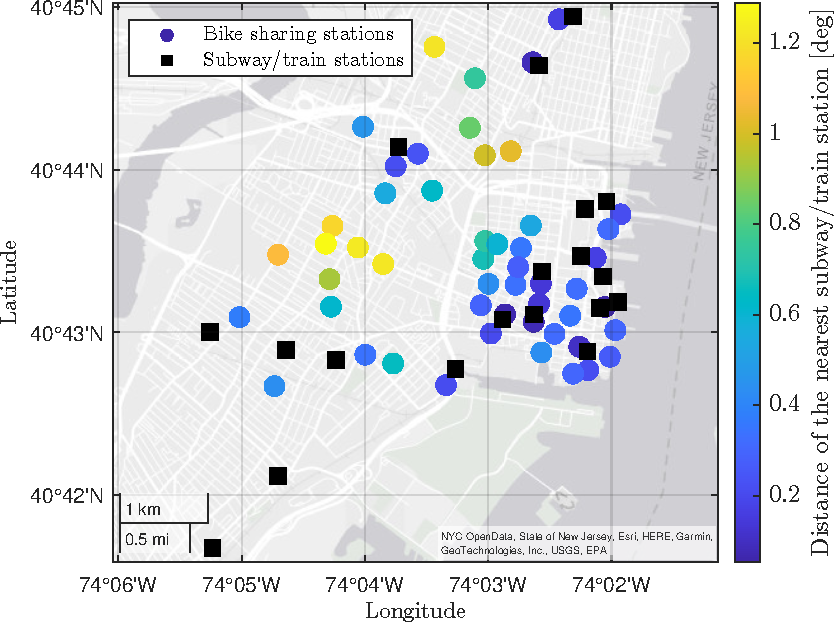
\includegraphics[height=172px]{Images/Dataset description/Chosen/Distances_map}}\quad
	\subfigure[]{\label{Train_map}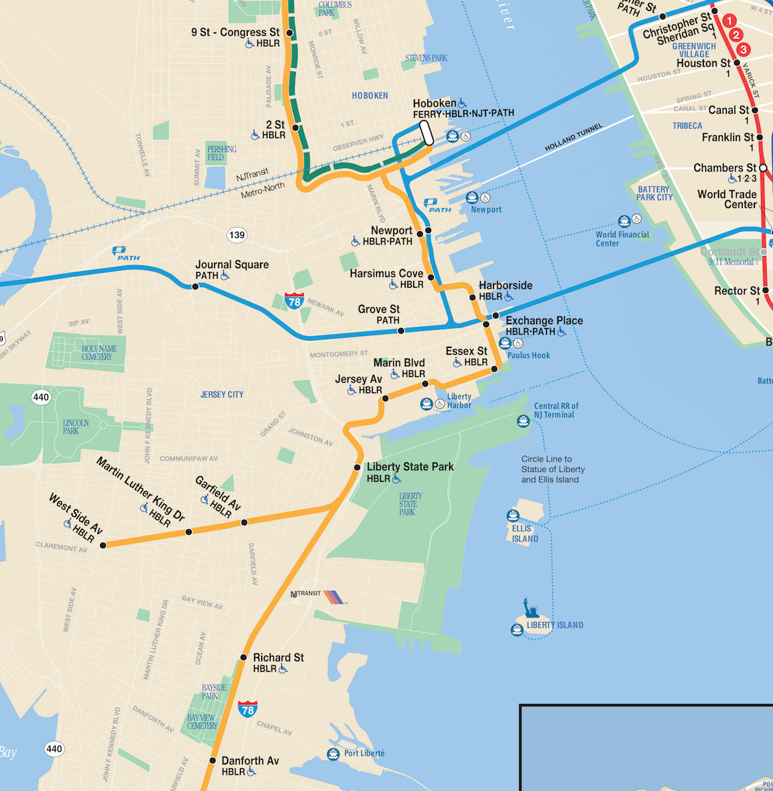
\includegraphics[height=172px]{Images/Dataset description/Chosen/Train_map}}\quad
	\caption[]{map of the bike rental stations and of the nearest subway/train stations (a) and map of the public transport network in Jersey City (b); in particular in blue it's indicated the path of the public transport service which reaches Manhattan, instead in yellow those which extends over the entire Jersey area.}
	\label{Maps}
\end{figure} 

\subsection{Weather variables}
The weather frequency variables that Visual Crossing provides to users with daily or hourly are:
\begin{itemize}
	\item \textbf{mean temperature}: in \unit{\degreeCelsius};
	\item \textbf{mean feels-like temperature}: in \unit{\degreeCelsius} (figure \ref{T_plot_box});
	\item \textbf{relative humidity}: in percentage;
	\item \textbf{rainfall}: in \unit{\milli\meter} (figure \ref{Rain_plot_box});
	\item \textbf{snowfall}: in \unit{\centi\meter};
	\item \textbf{mean wind speed}: in \unit{\kilo\meter/\hour};
	\item \textbf{cloud cover}: percentage of covered sky;
	\item \textbf{visibility}: maximum distance of visibility in \unit{\kilo\meter}. If the field of vision is greater than \SI{16}{\kilo\meter}, then the visibility value remains this one;
	\item \textbf{UV index}: indicates the energy of UV rays from \num{1} to \num{10}.
\end{itemize}
In table \ref{Weather_stats} we have summarized 

\begin{table}[h!]
	\centering
	\renewcommand\arraystretch{1.3}
	\begin{tabular}{c|c|c|c|c|c|c|c|c}
		\hline
		\textit{} & \textit{Min} & \textit{Max} & \textit{Mean} & \textit{Median} & \textit{Std} & \textit{Skew.}  & \textit{Kurt.} & \textit{R2} \\
		\hline
		\textbf{Temperature} & \num{-3.50} & \num{30.40} & \num{14.55} & \num{14} & \num{8.50} & \num{0.04} & \num{1.86} & \num{0.67} \\
		\hline
		\textbf{Feels-like temp.} & \num{-7.70} & \num{33.30} & \num{13.81} & \num{13.90} & \num{9.80} & \num{0.04} & \num{1.96} & \num{0.66} \\
		\hline
		\textbf{Humidity} & \num{35.10} & \num{93.50} & \num{65.28} & \num{66.10} & \num{13.78} & \num{0.08} & \num{2.18} & $\sim 0$ \\
		\hline
		\textbf{Rainfall} & \num{0} & \num{31.03} & \num{1.11} & \num{0} & \num{3.44} & \num{5.44} & \num{39.01} & \num{-0.06} \\
		\hline
		\textbf{Snowfall} & \num{0} & \num{157.50} & \num{0.78} & \num{0} & \num{9.61} & \num{14.45} & \num{219.19} & \num{-0.05} \\
		\hline
		\textbf{Wind speed} & \num{9.90} & \num{47.80} & \num{20.64} & \num{19.90} & \num{6.89} & \num{0.98} & \num{3.90} & \num{-0.26} \\
		\hline
		\textbf{Cloud cover} & \num{0.10} & \num{100} & \num{39.45} & \num{37.15} & \num{29.79} & \num{0.35} &\num{ 1.95} & \num{-0.33} \\
		\hline
		\textbf{Visibility} & \num{6.50} & \num{16} & \num{15.29} & \num{16} & \num{1.54} & \num{-2.99} & \num{12.83} & \num{0.24} \\
		\hline
		\textbf{UV index} & \num{ 0} & \num{10} & \num{5.92} & \num{6} & \num{2.88} & \num{-0.21} & \num{1.84} & \num{0.46} \\
		\hline
	\end{tabular}
	\caption{main statistics concerning weather variables. The R2 index describes the linear correlation between a meteorological covariate and the mean number of daily pickups.}
	\label{Weather_stats}
\end{table}

\begin{figure}[h!]
	\centering
	\subfigure[]{\label{T_plot_box}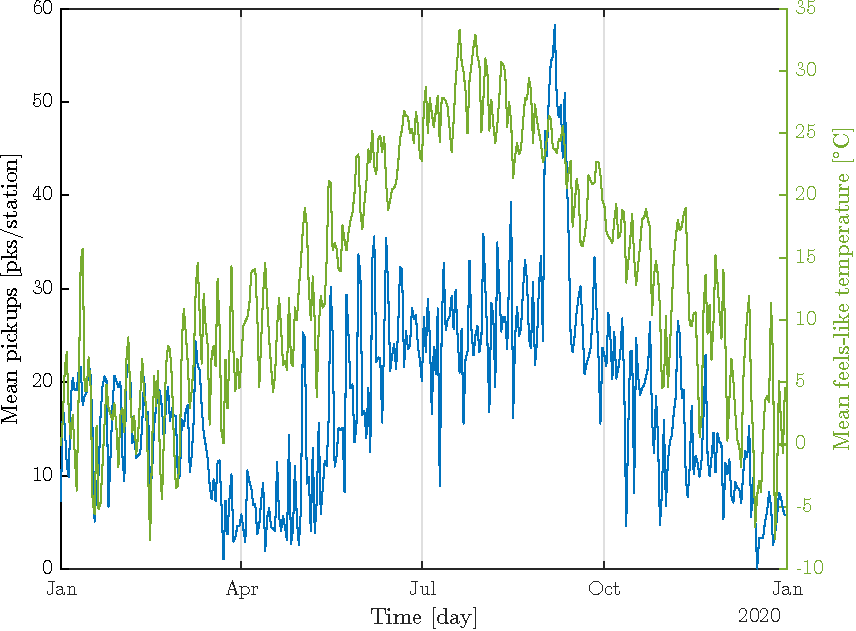
\includegraphics[height=172px]{Images/Dataset description/Chosen/Mean_feels_like_temperature_plot}}\quad
	\subfigure[]{\label{Rain_plot_box}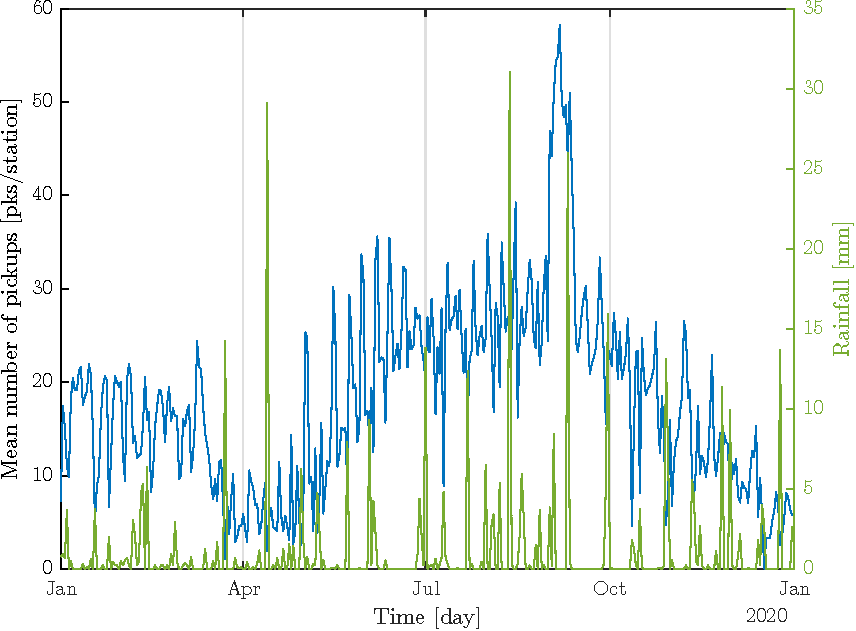
\includegraphics[height=172px]{Images/Dataset description/Chosen/Rainfall_plot}}\quad
	\subfigure[]{\label{T_box}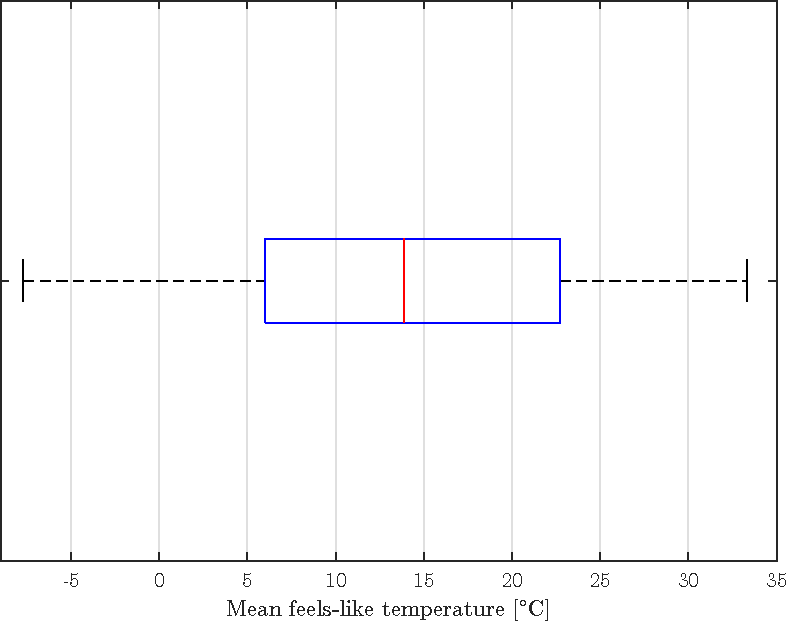
\includegraphics[height=172px]{Images/Dataset description/Chosen/Mean_feels_like_temperature_box}}\quad
	\subfigure[]{\label{Rain_box}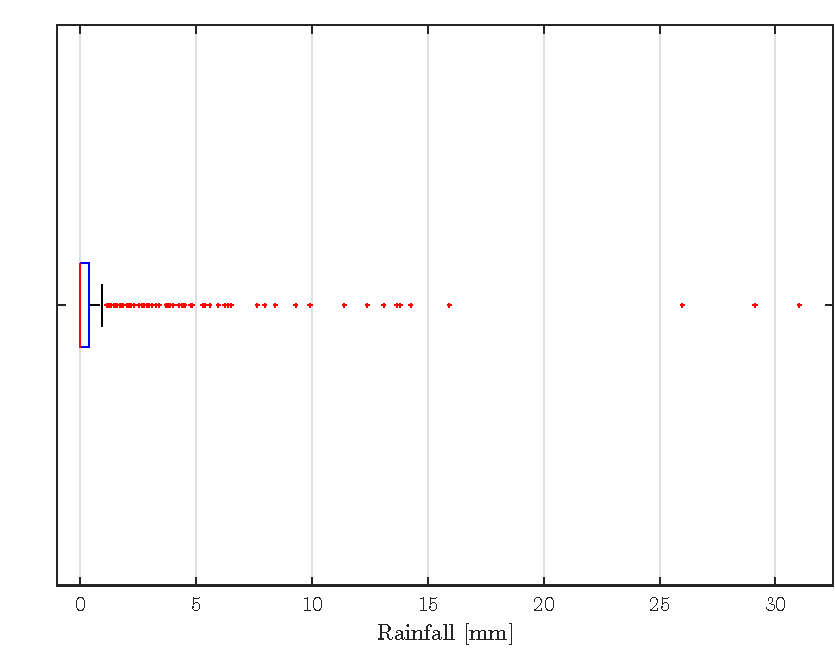
\includegraphics[height=172px]{Images/Dataset description/Chosen/Rainfall_box}}\quad
	\subfigure[]{\label{Cloud_box}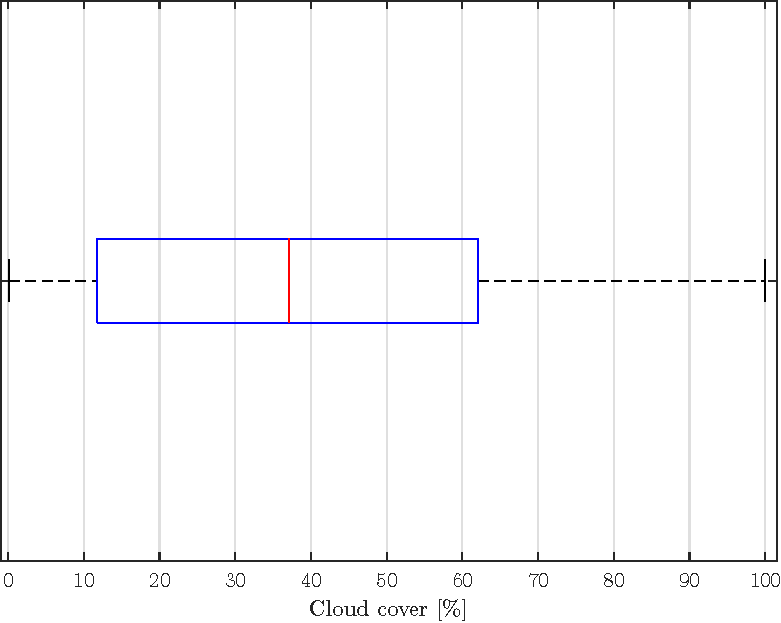
\includegraphics[height=172px]{Images/Dataset description/Chosen/Cloud_cover_box}}\quad
	\subfigure[]{\label{UV_box}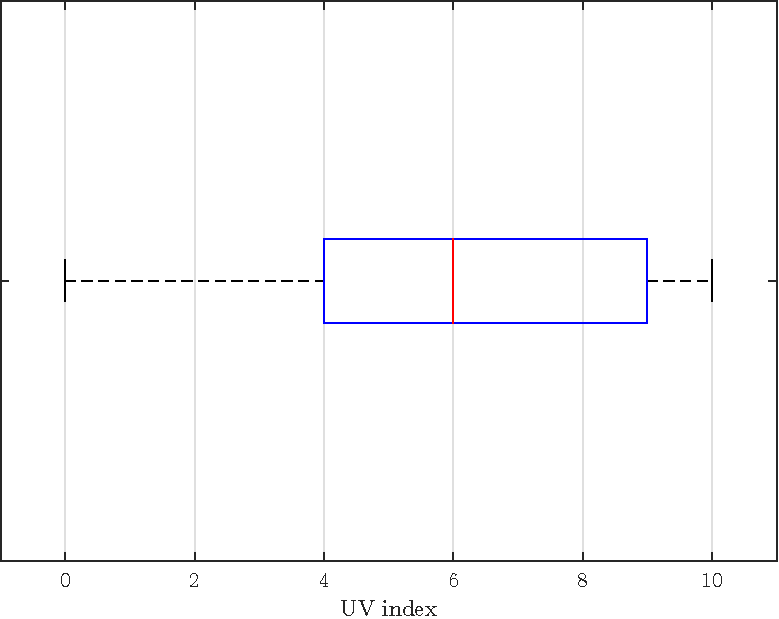
\includegraphics[height=172px]{Images/Dataset description/Chosen/UV_index_box}}\quad
	\caption{On the top left and right, there is the trend of two bike sharing variables, the pickups per station in blue and the average trip duration in dotted red line. On bottom there is the trend of two weather variables in green line, on left is indicated the average feels-like temperature, on right there is the rainfall. The light red patch describes the lockdown period. It is easy to observe that the weather variables have a strong influence, in particular the temperature has a positive effect on the rentals, on the contrary the amount of rainfall has a negative impact. Unfortunately the lockdown breaks these considerations, probably because many people didn't have the possibility to rent a bike}
\end{figure}

\subsection{Dummy variables}
As already mentioned, we hypothesize that some events may influence the demand for bike rentals, especially the presence of lockdowns or the presence of public holidays. So we have defined the following binary dummy variables:
\begin{itemize}
	\item \textbf{lockdown}: this is equal to \num{1} if there are restrictions in New York City, due to Covid and \num{0} if there are none;
	\item \textbf{holidays}: is equal to \num{1} when it is Saturday, Sunday or when there is a public holiday, \num{0} on the remaining days.
\end{itemize}

\begin{figure}[h!]
	\centering
	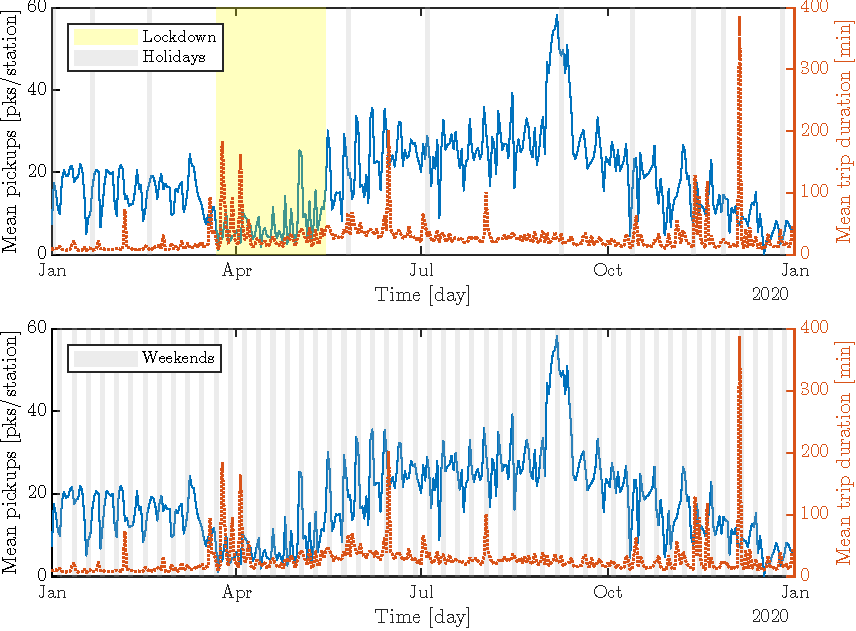
\includegraphics[height = 200px]{Images/Dataset description/Chosen/Trend}
\end{figure}